\documentclass{article}
\usepackage[utf8]{inputenc}
\usepackage{abstract}
\usepackage{hyperref}
\usepackage[super,square]{natbib}%%%参考文献引用格式调整
\renewcommand{\abstractnamefont}{\Large\bfseries}
\parindent=19pt
\usepackage{latexsym,bm,amsmath,amssymb}
\title{\textbf{Simple Saliency Detection based on LR-model with Laplacian\- 
		matrix}}
\author{Yongqi Yuan,Zhe Chen}
\date{November 2020}
\usepackage{listings}
\usepackage{natbib}
\usepackage{graphicx}
\usepackage{xcolor}

\lstset{
	%backgroundcolor=\color{red!50!green!50!blue!50},%代码块背景色为浅灰色
	rulesepcolor= \color{gray}, %代码块边框颜色
	breaklines=true,  %代码过长则换行
	numbers=left, %行号在左侧显示
	numberstyle= \small,%行号字体
	%keywordstyle= \color{blue},%关键字颜色
	commentstyle=\color{gray}, %注释颜色
	frame=shadowbox%用方框框住代码块
}
\begin{document}

\maketitle

\begin{abstract}
The low rank restoration model shows the potential of salient target detection, in which one matrix is decomposed into a low rank matrix representing the image background and a sparse matrix for recognizing the prominent target. However, there are still two defects. First, previous work usually assumes that the elements in the sparse matrix are independent of each other, which ignores the relationship between space and pattern in the image region. Secondly, when the low rank matrix and the sparse matrix are related, it is difficult to separate them from each other. In this paper, we propose a new structure of regularization model to enlarge the gap between these two models. In addition, advanced prior knowledge is integrated to guide matrix decomposition and improve detection efficiency. \citep{2017Salient}Our group has implemented the Laplace regularization method in matlab code, and has carried on the case study in the aspect of image saliency detection.
\end{abstract}

\section{Introduction}
In recent years, salience detection is a hot research topic.For a large data matrix, how to extract the characteristic information in it is a key point.Many people put forward their own methods in this aspect, among many methods, low-rank matrix recovery model is widely used in data dimension reduction and salience detection because of its good characteristics. If the laplacian regularization is added to the LR-model results,it can improve the effect of detection a lot.This paper bases on the previous research on significant detection, we use MATLAB to realize laplacian-matrix LR-model, and we analyze and study the experimental results.

For a nonnegative matrix, we have a decomposition method,$$X = UV^T.$$ in order 
to preserve the spatial structure, Cai,he et al.Proposed the gnmf 
model,\citep{2011Graph} namely min $$\| X-UV^T\|^2+\lambda*tr(V^TLV),$$ which 
enables the image in the new space to retain its spatial structure in the 
original space. The combination of the above two is the initial idea of SMD 
model. We will combine LR model with gnmf idea and carry out experimental 
analysis.
\section{Problem statement }
Given an image I, it is first partitioned into N non-overlapping patches 
$P=\{P_1,P_2, \cdots ,P_N\}$. For each patch $P_i$ a D-dimension row vector is 
reshaped and denoted as $x_i \in \mathbb{R}^D$, where $D=ws \times ws$ where 
$ws$ means the length of side of $P_i$ which is a square shaped square. And the 
whole matrix $X$ can be written as $X=\left[x_a,x_2,\cdots,x_n\right]\in 
\mathbb{R}^{D \times N}$. The problem of salient object detection based 
LR-model is to effectively decompose the patch matrix $X$ into a redundant 
information part $L$ (the non-salient background) and a sparse part $S$ (the 
salient foreground). The LR-model can be written as:
$$
min \ \|L\|_{*}+ \lambda \|S\|_1 
$$
$$
s.t.\ X=L+S
$$
And this one is the first model, the second model which is from the idea we got 
from $SMD$ model can be written as:
$$
min \ \|L\|_{*}+ \lambda \|S\|_1 + \beta Tr(SM_FS^T) 
$$ 
$$
s.t.\ X=L+S
$$
Here the $M_F$ is the Laplacian matrix, which is from the $GNMF$ model. 
Actually, if we write the matrix exactly, it can be written as:
$$
Tr(SM_FS^T)=\frac{1}{2} \sum_{i,j=1}^{N}\|x_i-x_j\|^2_2w_{i,j}
$$
where $x_i$ denotes the $i-th$ row of X, $w_{i,j}$ is the $(i,j)-th$ entry of 
an affinity matrix $W=(w_{i,j}\in \mathbb{R}^{N\times N})$ and represents the 
feature similarity of patches $(P_i,P_j)$, specially the affinity matrix W is 
defined as:$$w_{i,j}=exp(-\frac{\|x_i-x_j\|^2}{2\sigma ^2})$$
that's all what we are familiar with. So it's time to solve the models to get 
the salient object from the input image I.
\subsection{Optimization to LR-model}
Considering the balance between efficiency and accuracy in practice, we resort 
to the alternating direction method(ADM) to solve the convex problem in 
LR-model. And the model can be written as:
$$
min \ \|L\|_{*}+\lambda\|S\|_1+<Y,X-L-S>+\frac{\mu}{2} \|X-L-S\|^2_F
$$
where Y is the Lagrange multiplier, and $\mu>0$ controls the penalty for 
violating the linear constraints. To solve the above equation, we search for 
the optimal L and S iteratively, and in each iteration the two components are 
updated alternately.\\
\textbf{Updating S:}minimal S with other variables fixed :
$$
\underset{S}{min} \ \lambda\|S\|_1+<Y,X-L-S>+\frac{\mu}{2}\|X-L-S\|^2_F
$$
So here we have:
$$
S=\underset{S}{argmin} \ 
\frac{\lambda}{\mu}\|S\|_1+\frac{1}{2}\|S-(X-L+\frac{Y}{\mu})\|^2_F
$$
the solution of this model is:
$$
S=T_{\frac{\lambda}{\mu}}(X-L+\frac{Y}{\mu})
$$
where the $T_{\epsilon}(X)$ is the soft threshold operator:
$$ T_{\epsilon}(x)=
\left\{
\begin{aligned}
	x & \ \ - &\epsilon &, x>\epsilon\\
	x & \ \ + &\epsilon &, x<-\epsilon\\
	& \ \ 0 & \ &, otherwise
\end{aligned}
\right.
$$
\\
\textbf{Updating L:}minimal L with other variables fixed, so we have:
$$
\underset{L}{min}\ \|L\|_{*}+<Y, X-L-S>+\frac{\mu}{2}\|X-L-S\|^2_F
$$
after doing some transformation, we'll get:
$$
L=\ \underset{L}{argmin}\ 
\frac{1}{\mu}\|L\|_{*}+\frac{1}{2}\|L-(X-S+\frac{Y}{\mu})\|_F^2
$$
the solution of this equation is:
$$
L=UT_{\frac{1}{\mu}}(S)V^T
$$
where S is the singular value decomposition matrix of $X-S+\frac{Y}{\mu}$
$$
USV^T=SVD(X-S+\frac{Y}{\mu})
$$ 
\subsection{Optimization to laplacian-matrix based LR-model}
Just like what we did in the optimization to LR-model, here we'll optimize the 
model laplacian-matrix based LR-model, but in this step we'll introduce an 
auxiliary variable H to better solve the model, we show this here:
$$
min \|L\|_{*}+\lambda\|S\|_{1}+\beta 
Tr(HM_FH^T)+Tr(Y^T_1(X-L-S))\\
$$
\begin{flalign*}
	+Tr(Y^T_2(S-H))+\frac{\mu}{2}(\|X-L-S\|^2_F+\|S-H\|^2_F)
\end{flalign*}
where the $Y_1$ and $Y_2$ are the Lagrange multipliers, so in the optimization 
process, we'll do like what we did with LR-model:\\
\textbf{Updating L:}\ with S and H fixed
$$
L=\underset{L}{argmin}\ \|L\|_{*}+Tr(Y^T_1(X-L-S))+\frac{\mu}{2}\|X-L-S\|^2_F
$$
after some transformation we'll get the solution:
$$
L=UT_{\frac{1}{\mu}}(S)V^T
$$
here the S is a diagonal matrix with the elements the singular value of 
$X-S+\frac{Y_1}{\mu}$.
\\
\textbf{Updating H:}\ with L and S fixed
$$
H=\underset{H}{argmin}\ \beta 
Tr(HM_FH^T)+Tr(Y_2^T(S-H))+\frac{\mu}{2}\|S-H\|^2_F
$$
after doing some transformation of the equation the solution can be written as:
$$
H=(\mu S+Y_2)(2\beta M_F+\mu I)^{-1}
$$
\noindent
\textbf{Updating S:}\ with L and H fixed
$$
S=\underset{S}{argmin}\ 
\lambda\|S\|_1+Tr(Y^T_1(X-L-S))+Tr(Y^T_2(S-H))+\frac{\mu}{2}(\|X-L-S\|^2_F+\|S-H\|^2_F)
$$
To solve this equation we have:
$$
S=\underset{S}{argmin}\ 
\frac{\lambda}{\mu}\|S\|_1+\frac{1}{2}\|X-L-S+\frac{Y_1}{\mu}\|^2_F+\frac{1}{2}\|S-H+\frac{Y_2}{\mu}\|^2_F
$$
after doing some derivation with the equation we get the solution:
$$
S=T_{\frac{\lambda}{\mu}}(X-L+\frac{Y_1}{\mu}-\frac{Y_2}{\mu}+H)
$$

That's all what we do to solve the two models and in the next part we'll talk 
the experiments we did. And first we'll show the algorithm we use to solve 
laplacian-matrix based LR-model.
\newpage
\section{Algorithm}
$
\overline{\qquad\qquad\qquad\qquad\qquad\qquad\qquad\qquad\qquad\qquad\qquad\qquad\quad}
\\Algorithm\ 1\ laplacian-matrix\ based\ LR-model
\\\underline{\qquad\qquad\qquad\qquad\qquad\qquad\qquad\qquad\qquad\qquad\qquad\qquad\quad}
\\\mbox{Input: Feature matrix D, parameters}\rho,\beta,
\\1:\mbox{Initialize}L^0=0, S^0=0, H^0=0, Y_{1}^0=0, Y_{2}^0=0, \\\mu^0=0.1,\mu_{max} =10^{10}, \rho= 1.1, and\ k = 0.
\\2:\mbox{While not converged do}
\\3:(\mu,S,V^T)=SVD(D-E^k+Y_{1}^k/\mu)
\\4:A^{k+1}=\mu*T_{1/\mu}(S)*V^T
\\5:H^{k+1}=(\mu^k*E^k+Y_{2}^k)*(2\beta*M_F+\mu^k*I)^{-1}
\\6:E^{k+1}=T_{\lambda/\mu}(D-A^{k+1}+Y_{1}^k/\mu^k-Y_{2}^k/\mu^k+H^{k+1})
\\7:Y_{1}^{k+1}=Y_{1}^k+\mu^k(D-A^{k+1}-E^{k+1})
\\8:Y_{2}^{k+1}=Y_{2}^k+\mu^k(E^{k+1}-H^{k+1})
\\9:\mu^{k+1}=min(\rho*\mu^{k+1},\mu_{max})
\\10:k=k+1
\\11:End\ While
\\12:Return\ L^k\ and\ S^k.
\\\underline{\qquad\qquad\qquad\qquad\qquad\qquad\qquad\qquad\qquad\qquad\qquad\qquad\quad}
$
\section{Experiments and result analysis}
\subsection{Experiment process}
First, we'll get some images noted as "a~h", and get the result of salient 
object detection with SMD model. Then, we'll input the images into our matlab 
functions and decompose them into two parts noted as "low-rank part" and 
"sparse part", and them get the "salient part" by the information we get from 
"sparse part". So, that's one input and five parts output.
\subsection{Evaluation metrics}
Here we'll use the rank of L to evaluate the quality of "low-rank part" we get, 
and use the proportion of non-zero numbers of S to evaluate the quality of 
"sparse part" we get.
\subsection{Results and analysis}

\begin{figure}[htbp]
	\centering
	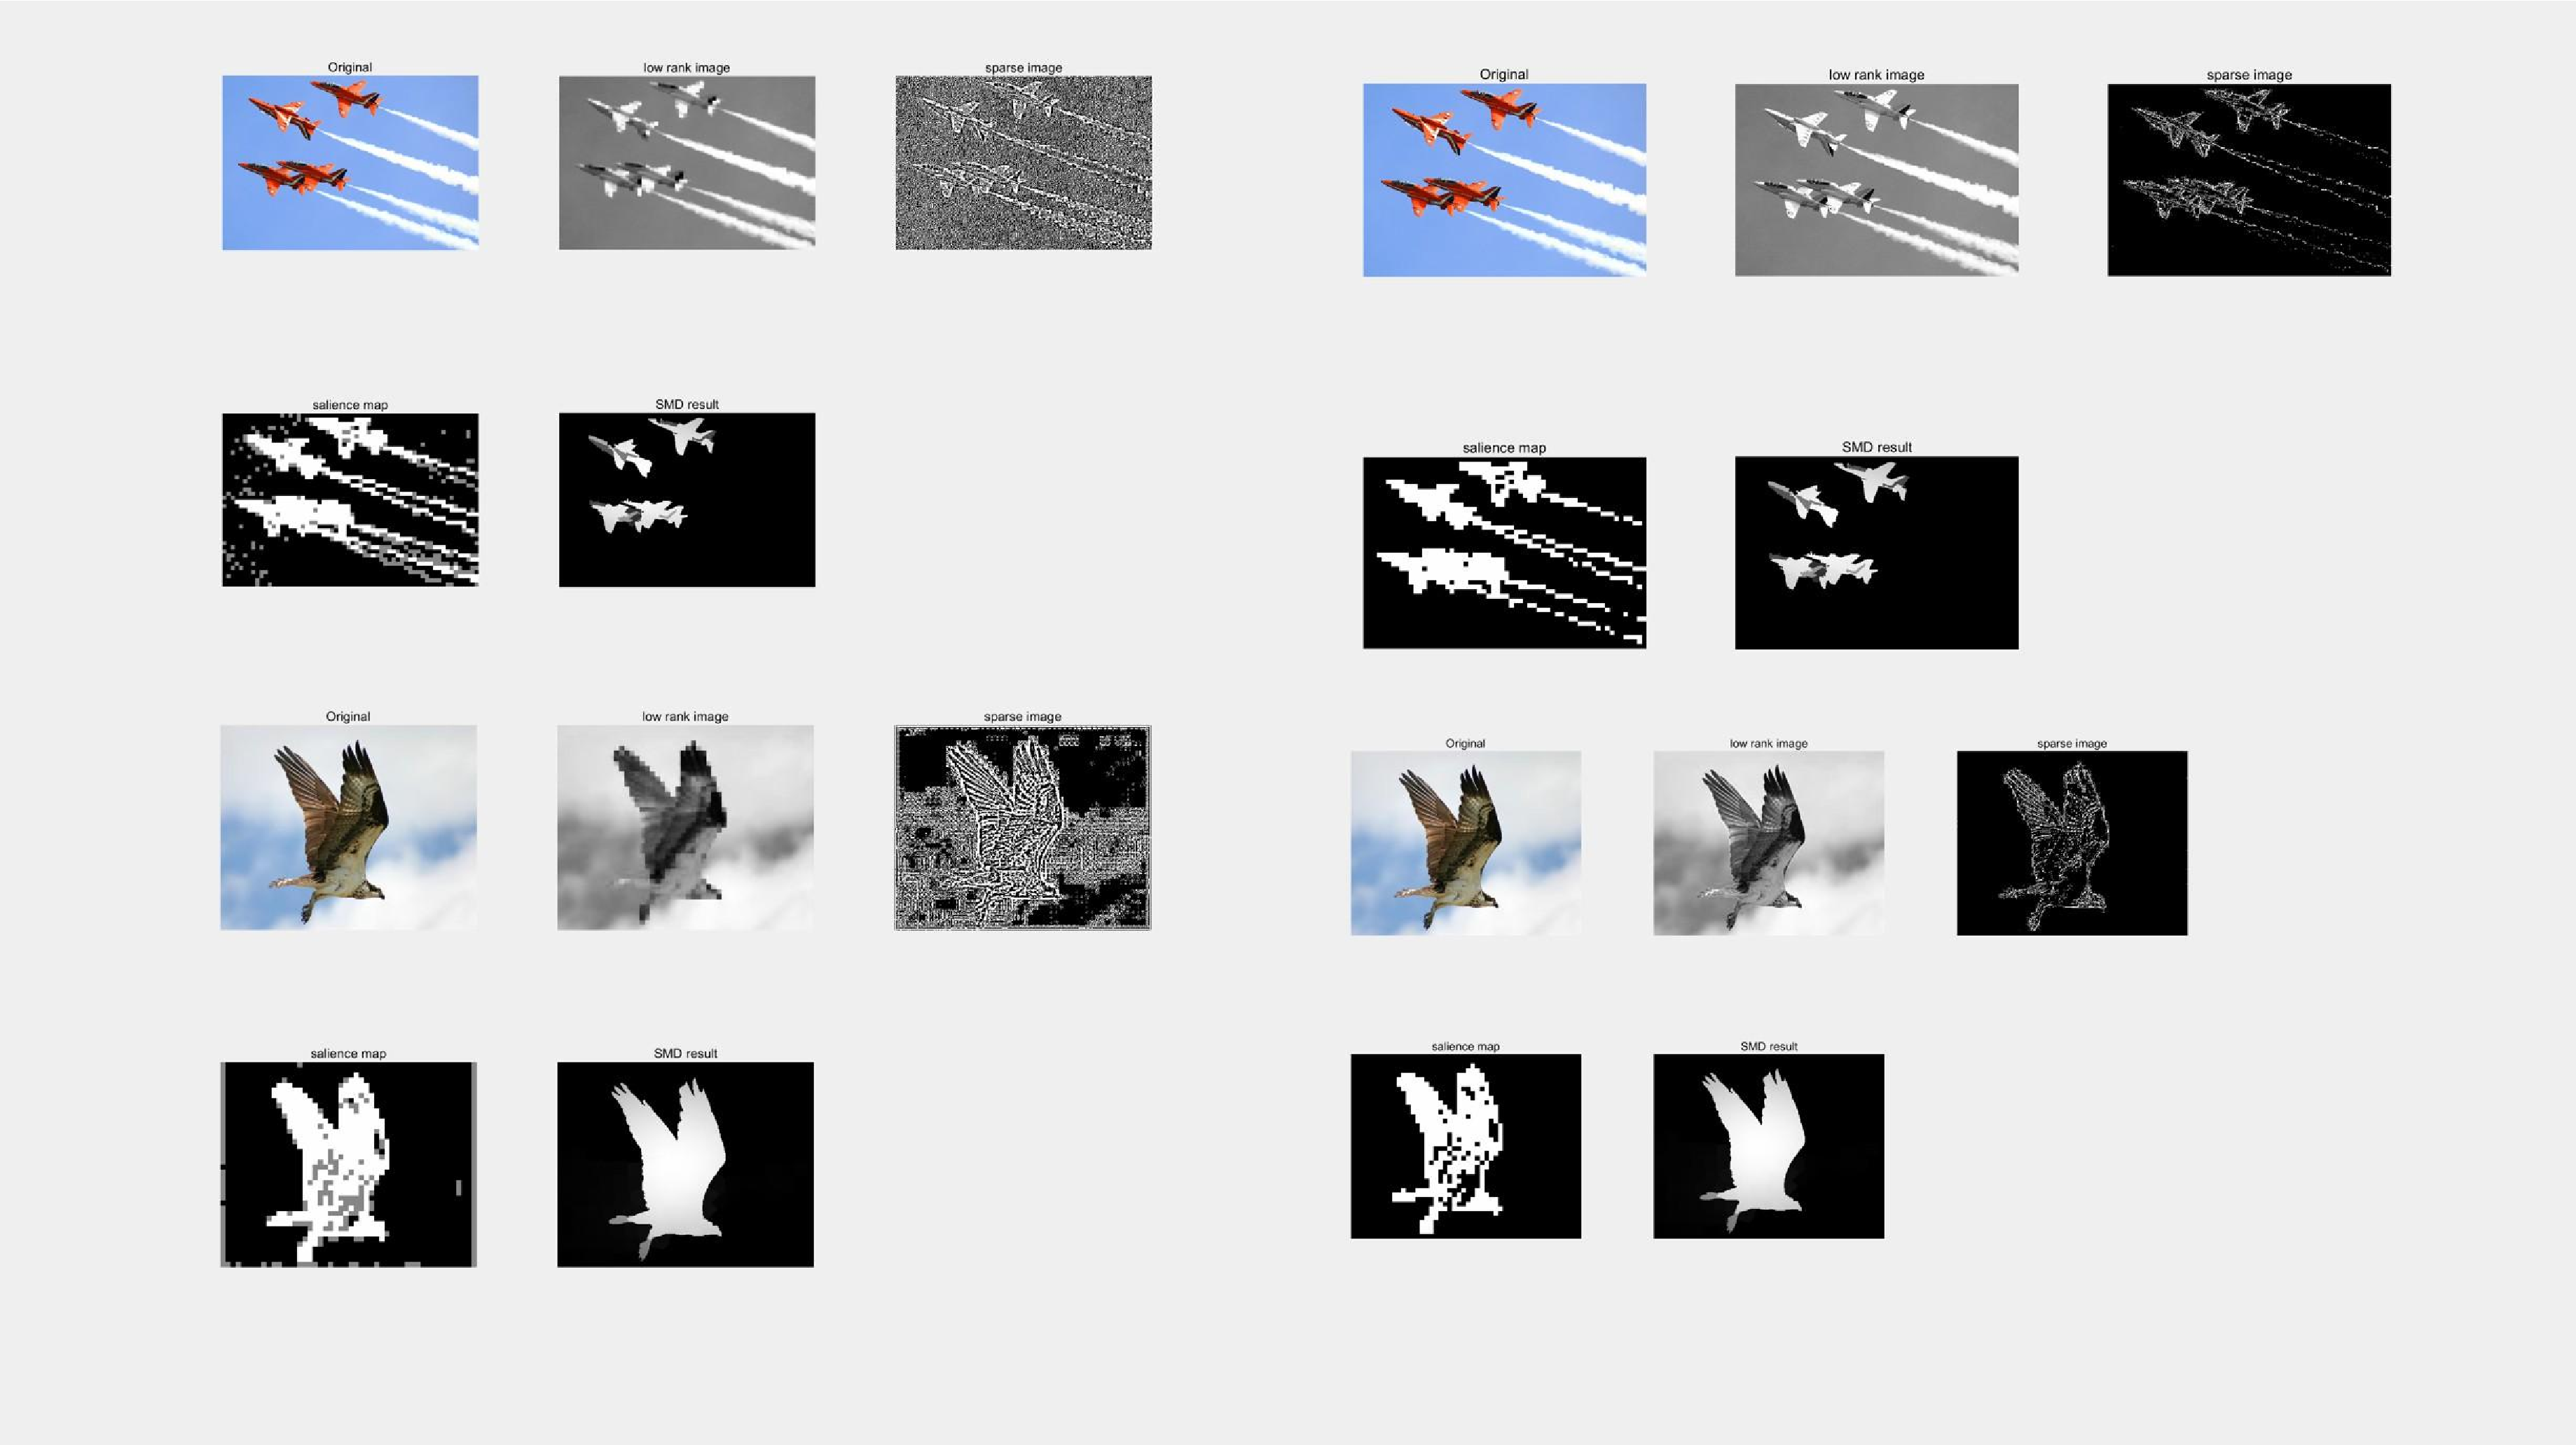
\includegraphics[width=0.95\textwidth]{result.pdf}
	\caption{Comparison between LR-model and laplacian-matrix based LR-model}
\end{figure} 

We can see the result of comparison between LR-model and laplacian-matrix based 
LR-model in Figure 1. The left two groups are the results from LR-model and the 
right groups are the results from laplacian-matrix based LR-model. For each 
group from the four groups, we input the original image which is in the first 
cell of each group, and the second, the third cells are the low-rank part, 
sparse part, the forth cell is the result generated from our own function and 
the fifth cell is the result generated from SMD-model. \\
First, we talk about the low-rank part. We can see clearly that every patches 
from the LR-model are fuzzy and some of them seem to be same. But the patches 
from the laplacian-matrix based LR-model are all totally different, which means 
they have a high even full rank. The exact numerical result is shown in Figure 
2 and Figure 3. 

\begin{figure}[htbp]
	\centering
	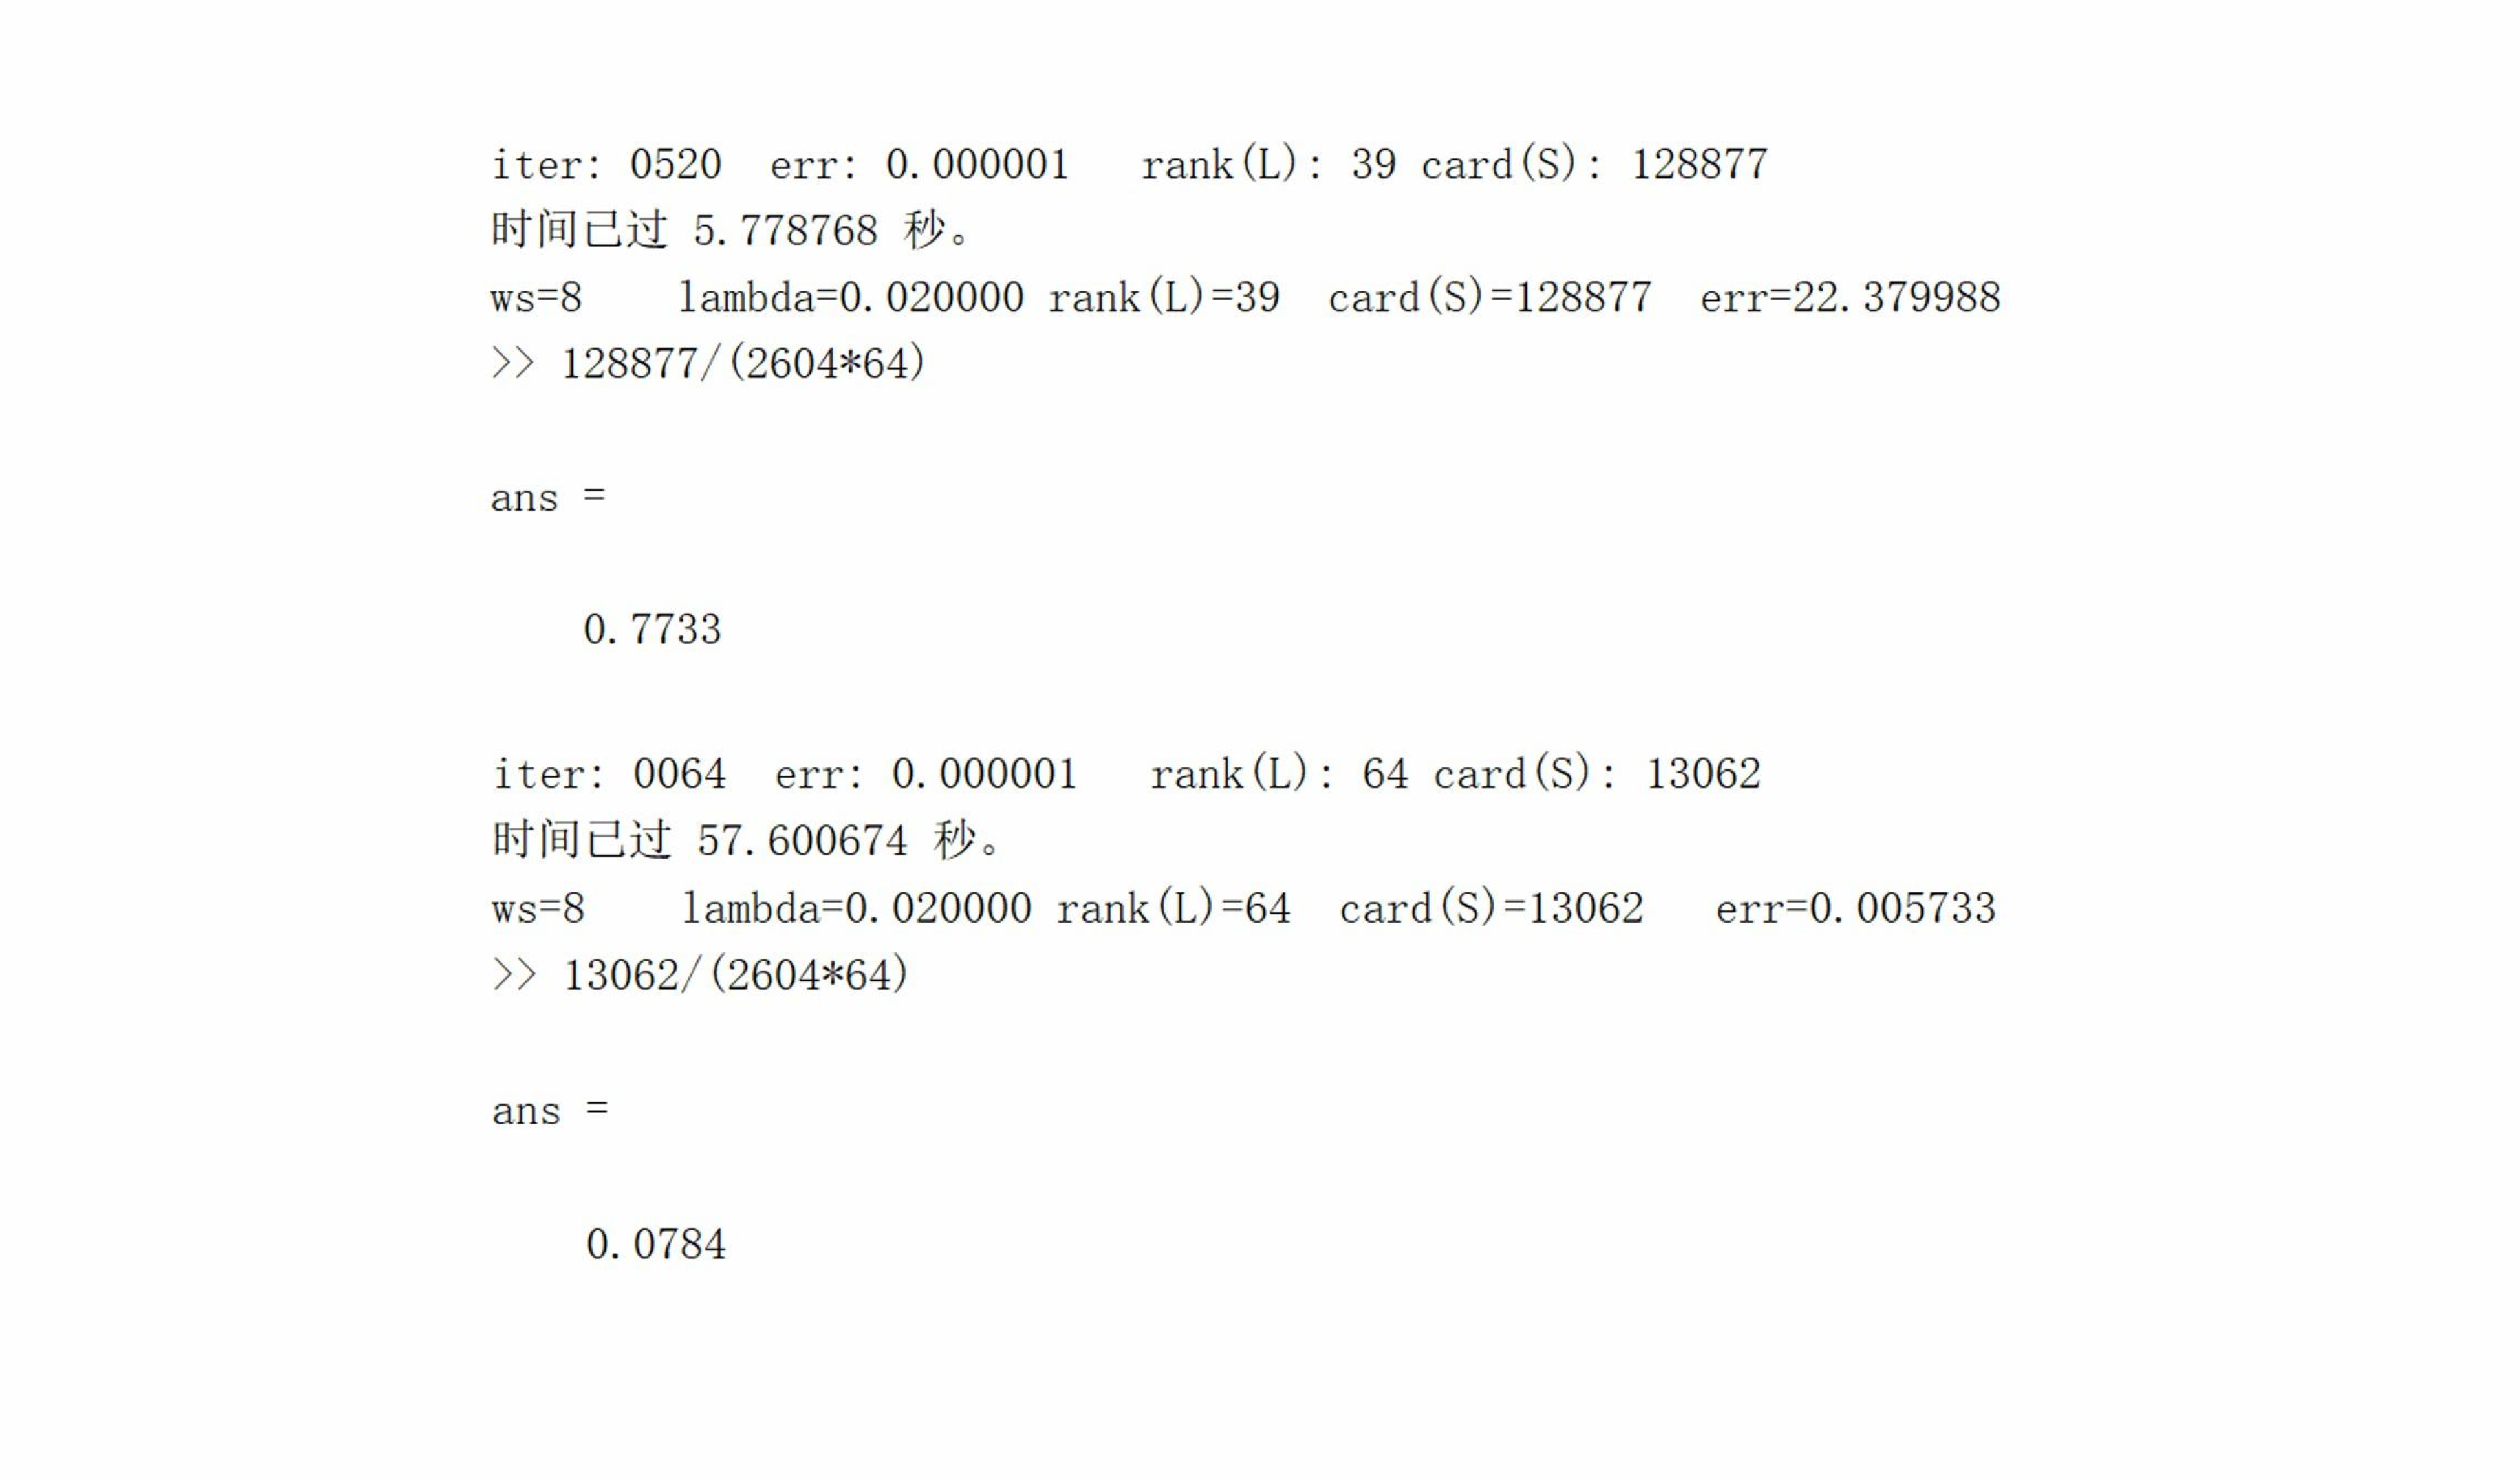
\includegraphics[width=0.70\textwidth]{img1result.pdf}
	\caption{Numerical result we got from the first image}
\end{figure} 
The above result is the LR-model result and underneath it the laplacian-matrix 
based LR-model. When we use the LR-model we can get a low rank result but a 
full rank result from the laplacian-matrix based LR-model. 
\begin{figure}[htbp]
	\centering
	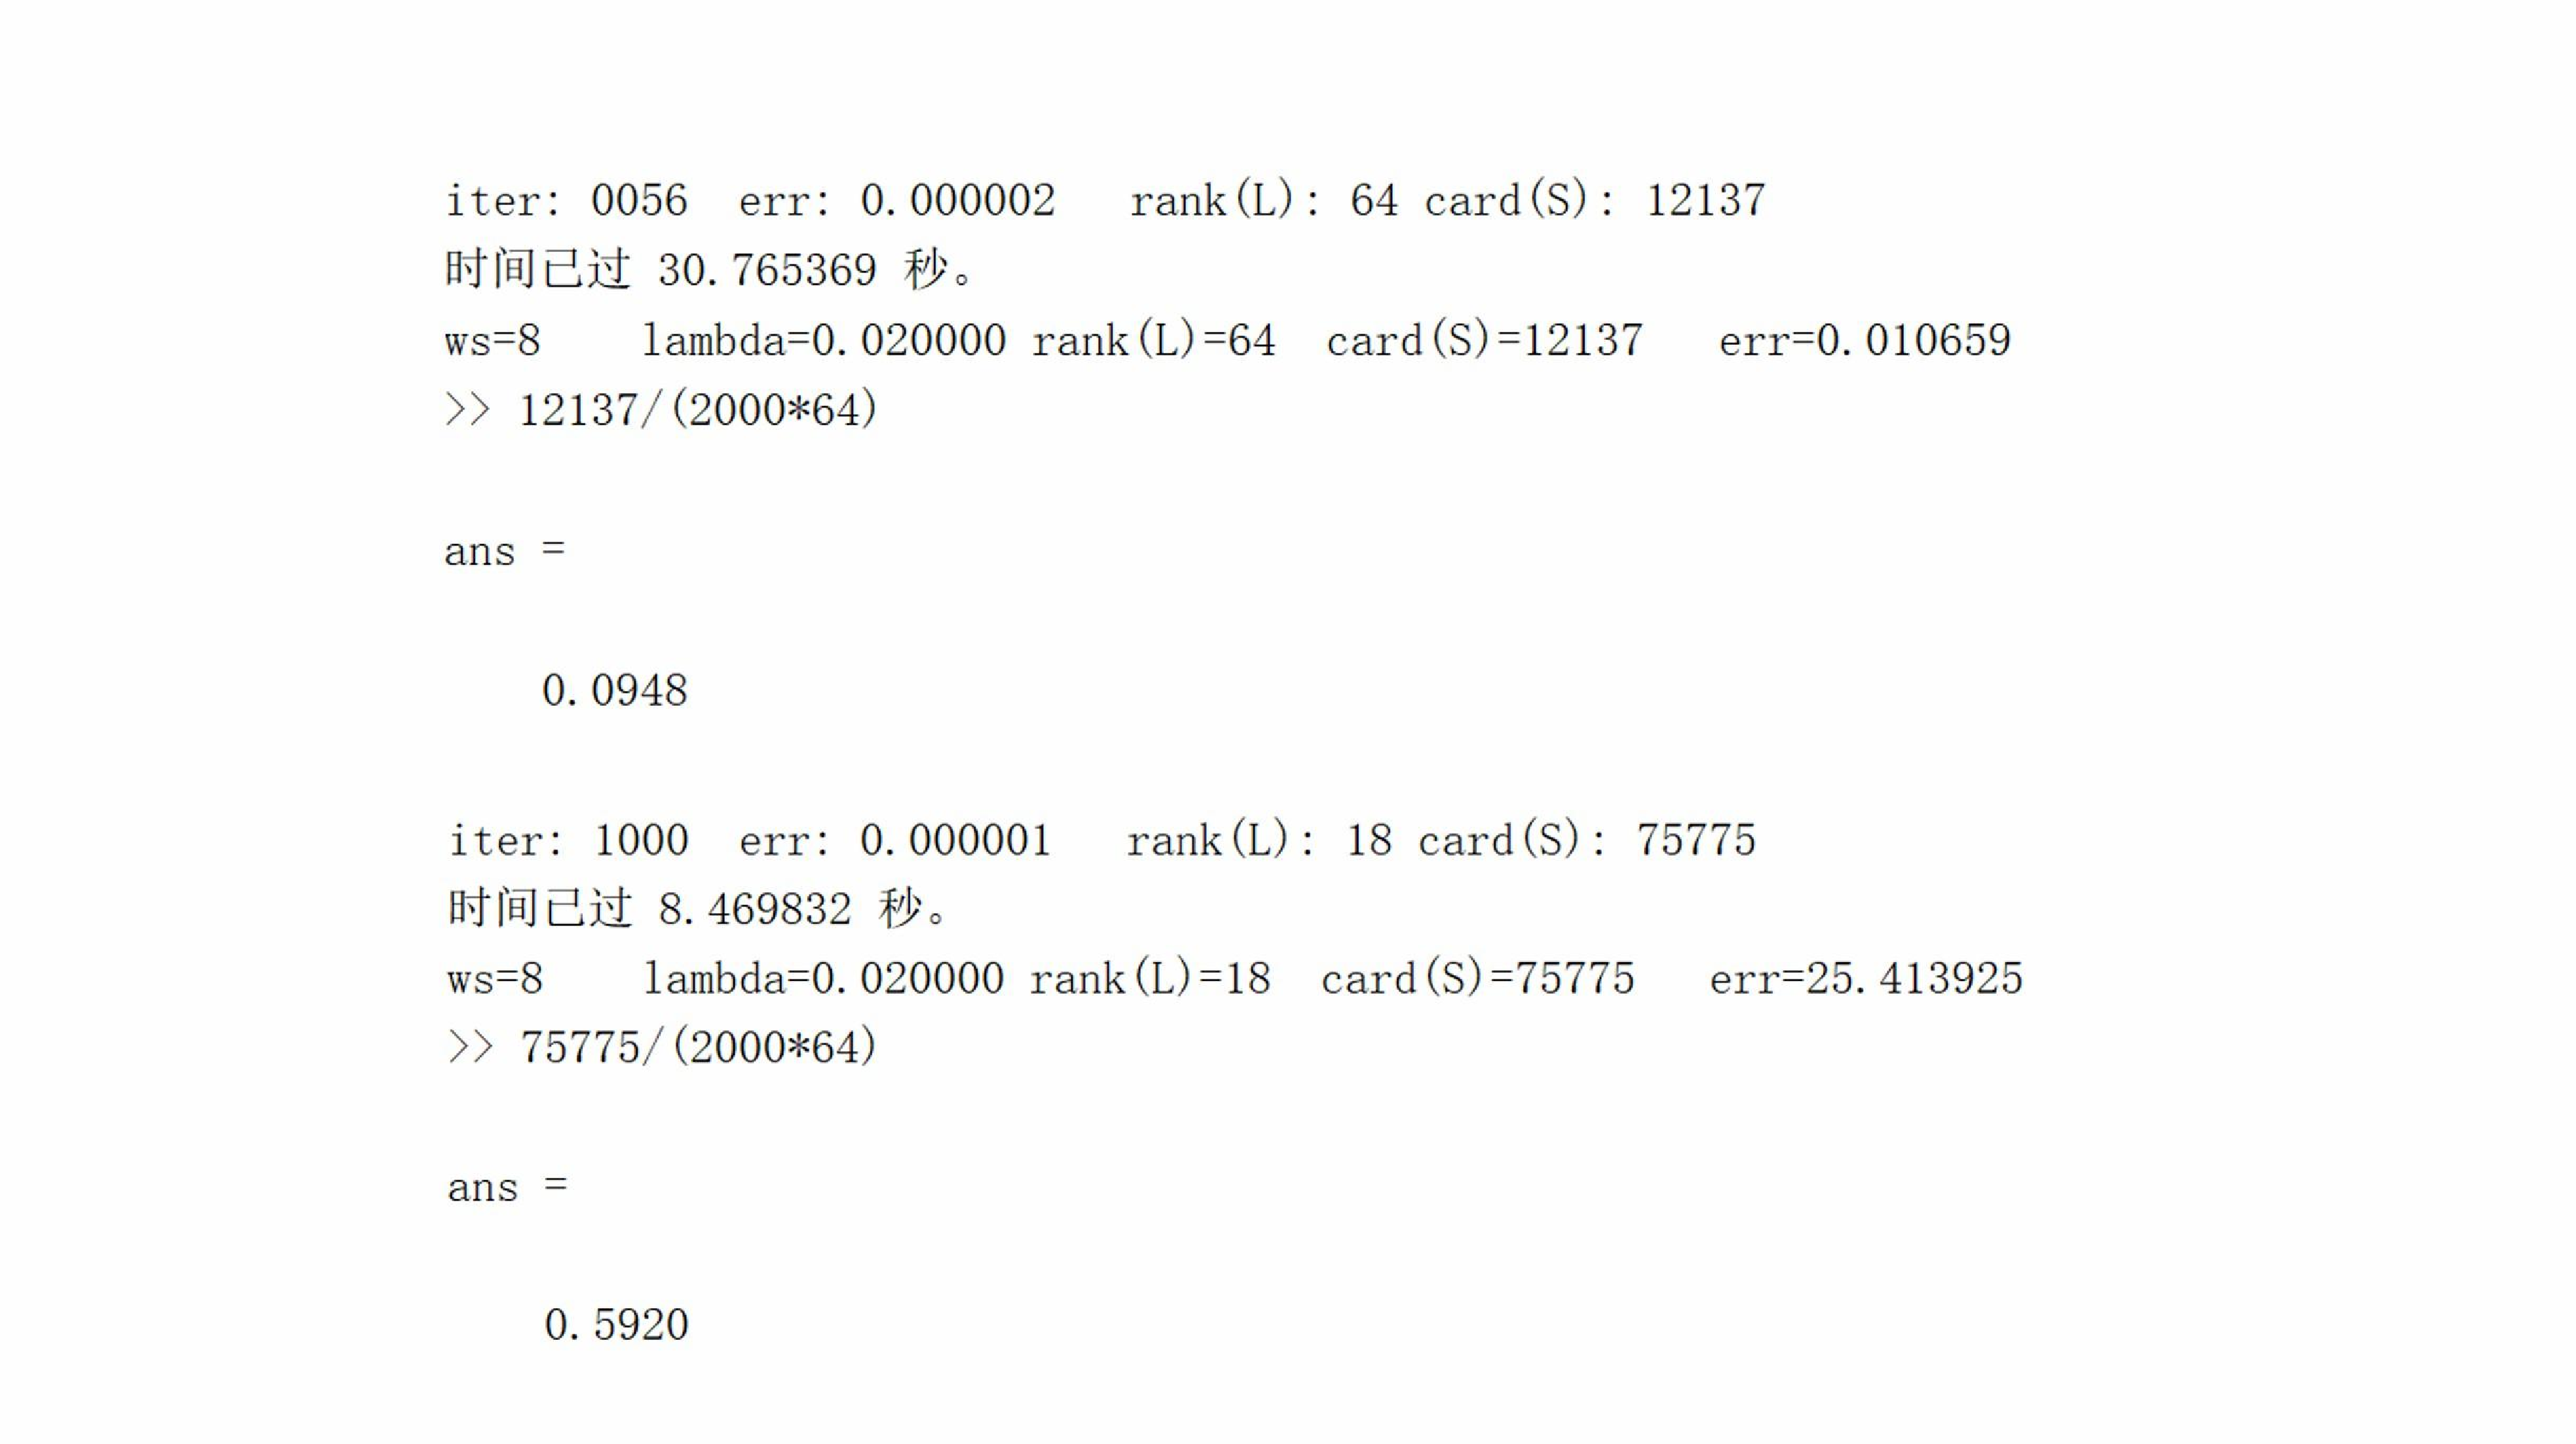
\includegraphics[width=0.70\textwidth]{img2result.pdf}
	\caption{Numerical result we got from the second image}
\end{figure}
And here we talk about the sparse part. In this part, we use the proportion of 
non-zero numbers to evaluate the quality of sparse part. The sparse part we get 
from the LR-model has a very big value of proportion which means it's not so 
sparse and we get a small value of proportion from the other model which means 
the opposite. \\
So we can get the first conclusion that LR-model can get a good result in 
low-rank, but poor quality in sparsity, and laplacian-matrix based LR-model can 
get a good result in sparsity but poor quality in low-rank. So the 
laplacian-matrix part plays an important role in separate the two parts but can 
not remain a good property in the low rank part.\\
The last part let's talk about the salient object we get. We use the 1-norm of 
each patches we get from the images'sparse part. We use quartile of the 1-norm 
rank of each image to do the evaluation. If the 1-norm is bigger than the three 
times of quartile, this patch's all pixels will be assigned a 255 value and so 
on. Because of the good property of the sparse part of laplacian-matrix based 
LR-model, we can see that we can also get a more salient result than the 
LR-model.\\
\subsection{Disadvantages of laplacian-matrix based LR-model}
From the results we get in the previous text, we can see that we'll get a very 
sparse result in the sparse part from the laplacian-matrix based LR-model. But 
sometimes we get a extremely sparse result such as Figure 4. 
\begin{figure}[htbp]
	\centering
	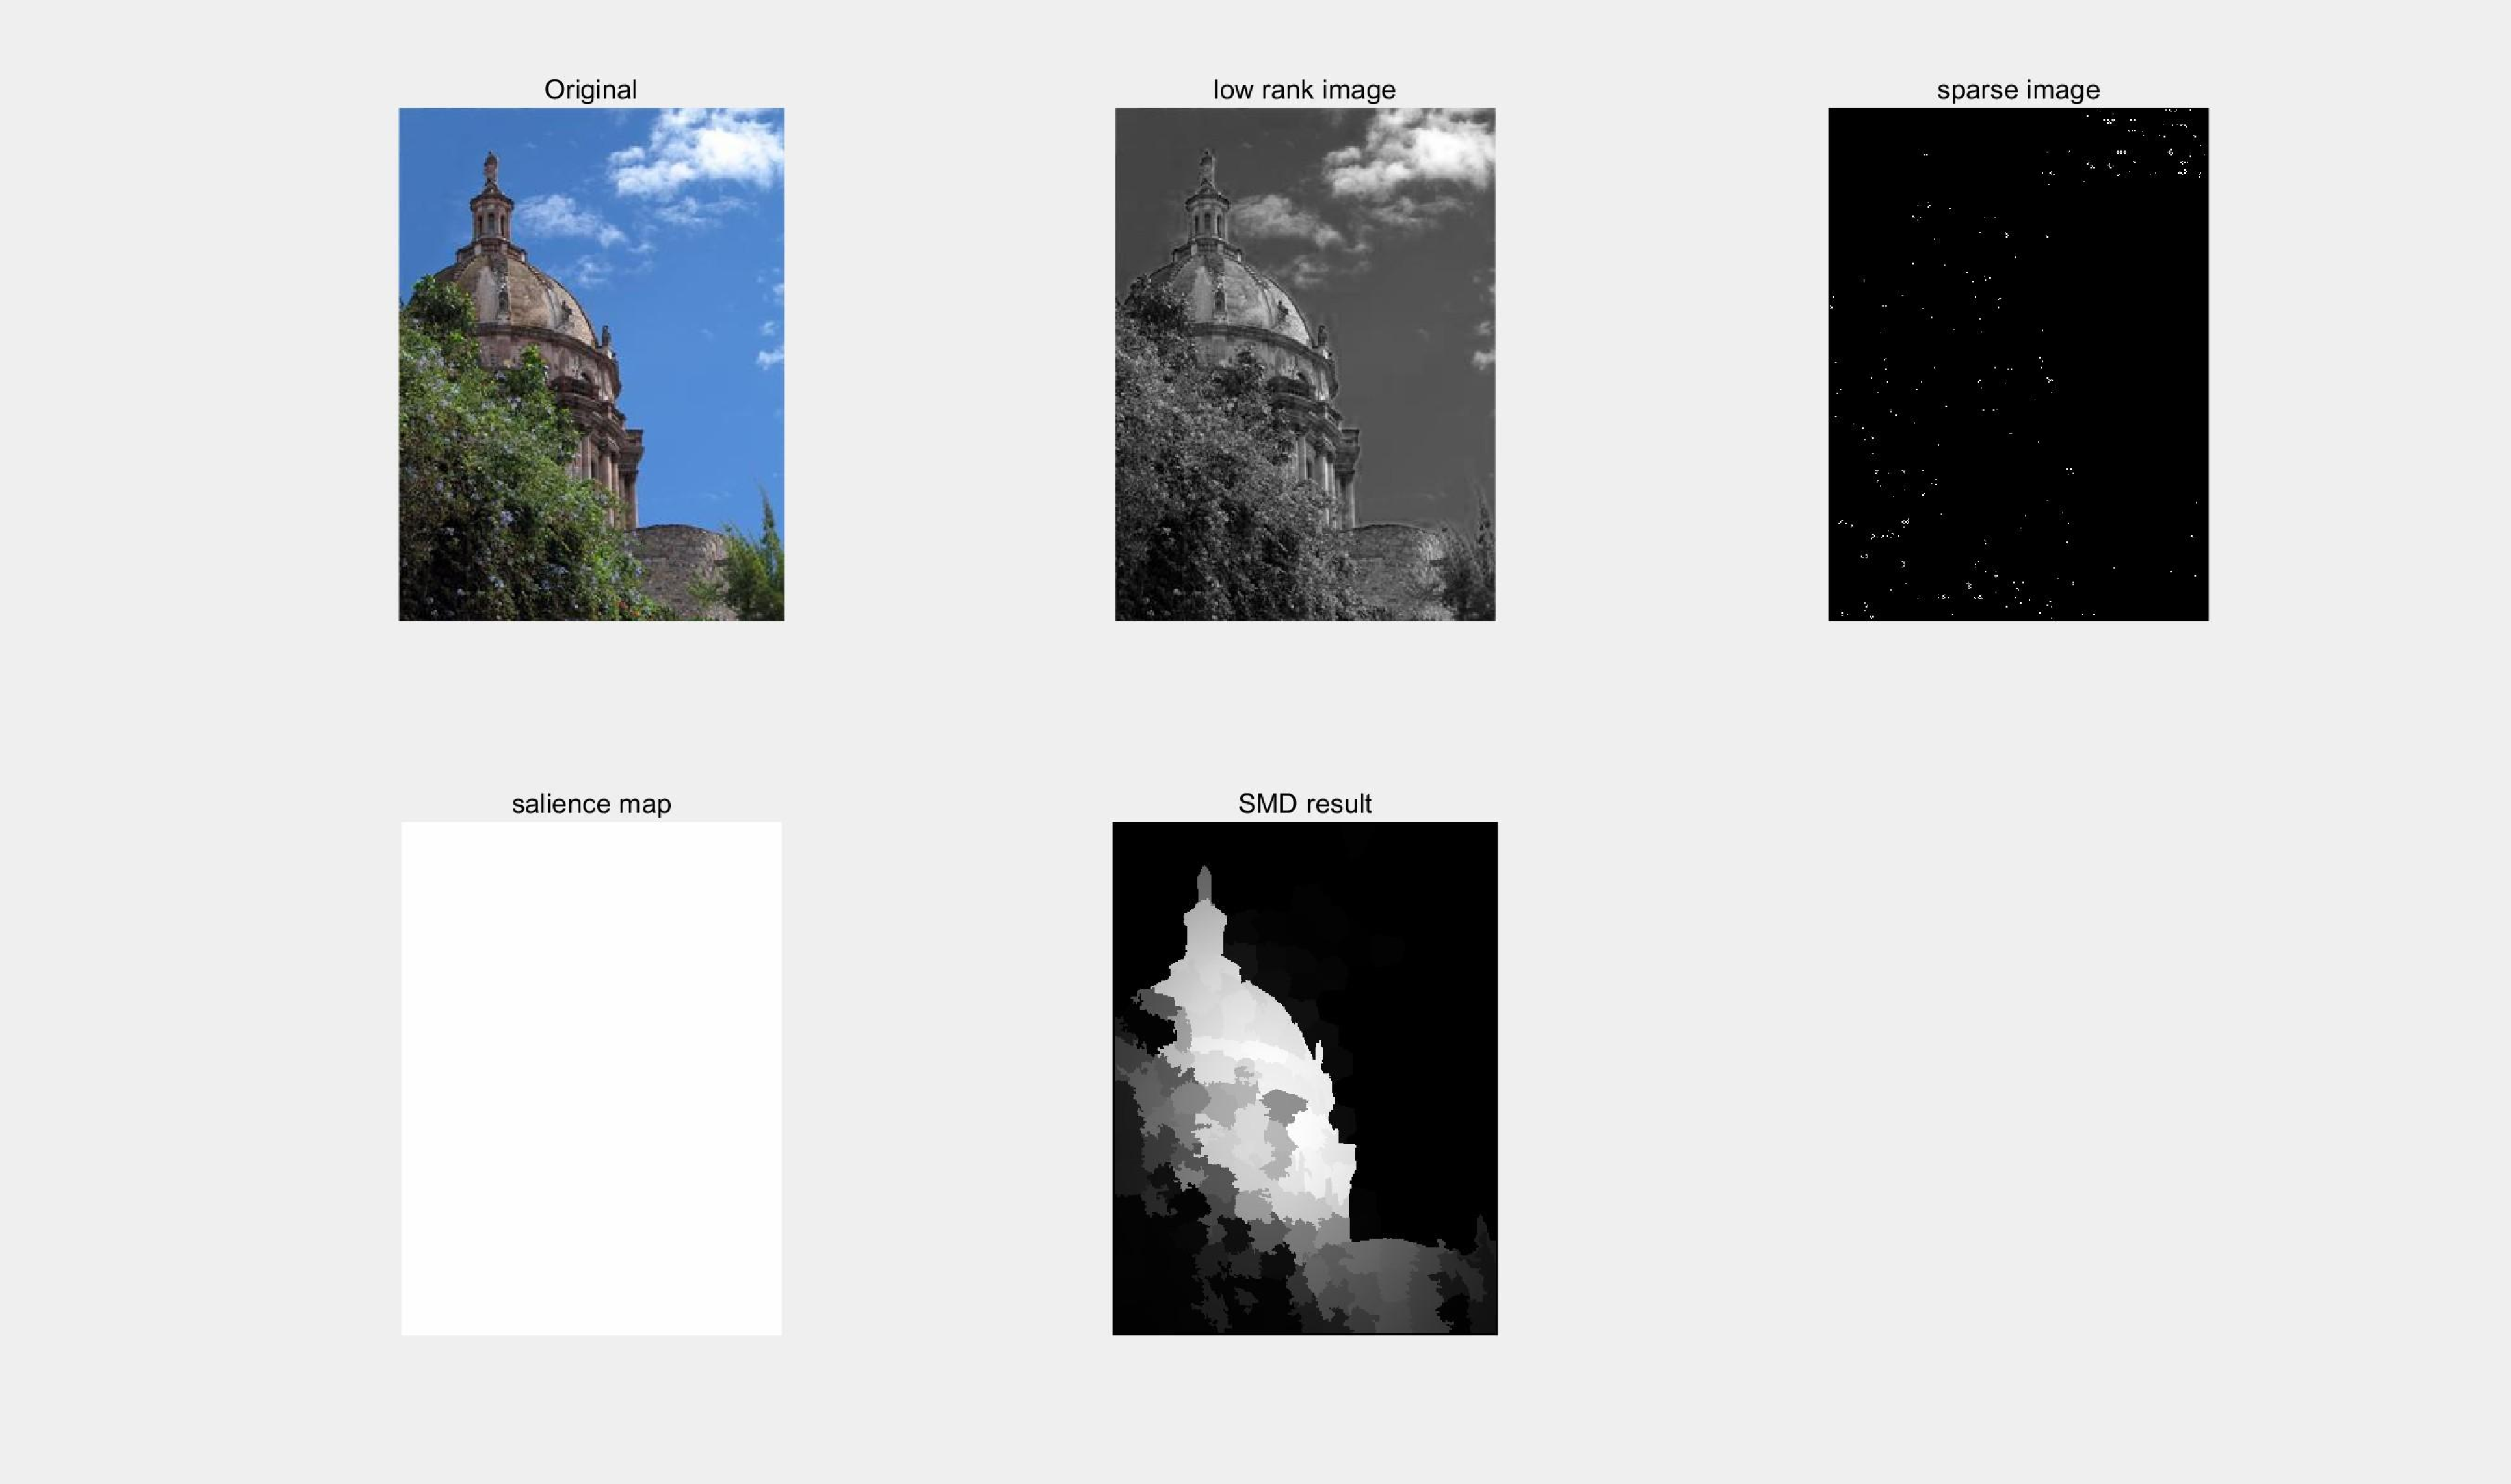
\includegraphics[width=0.95\textwidth]{strange.pdf}
	\caption{Numerical result we got from the second image}
\end{figure}
Because it's too sparse, so most of the sparse matrix elements are 0. And it 
leads all the quartiles are 0. So every elements are bigger than the quartiles 
which leads the pixels in the salient result all valued 255.\\
And we also found that we'll get a error explosion in the process of 
laplacian-matrix based LR-model decomposition. It's shown in the Figure 5. And 
this is a feature work we'll do, we just found that the mpower function in 
matlab has something wrong, so this is a feature work.


\begin{figure}[htbp]
	\centering
	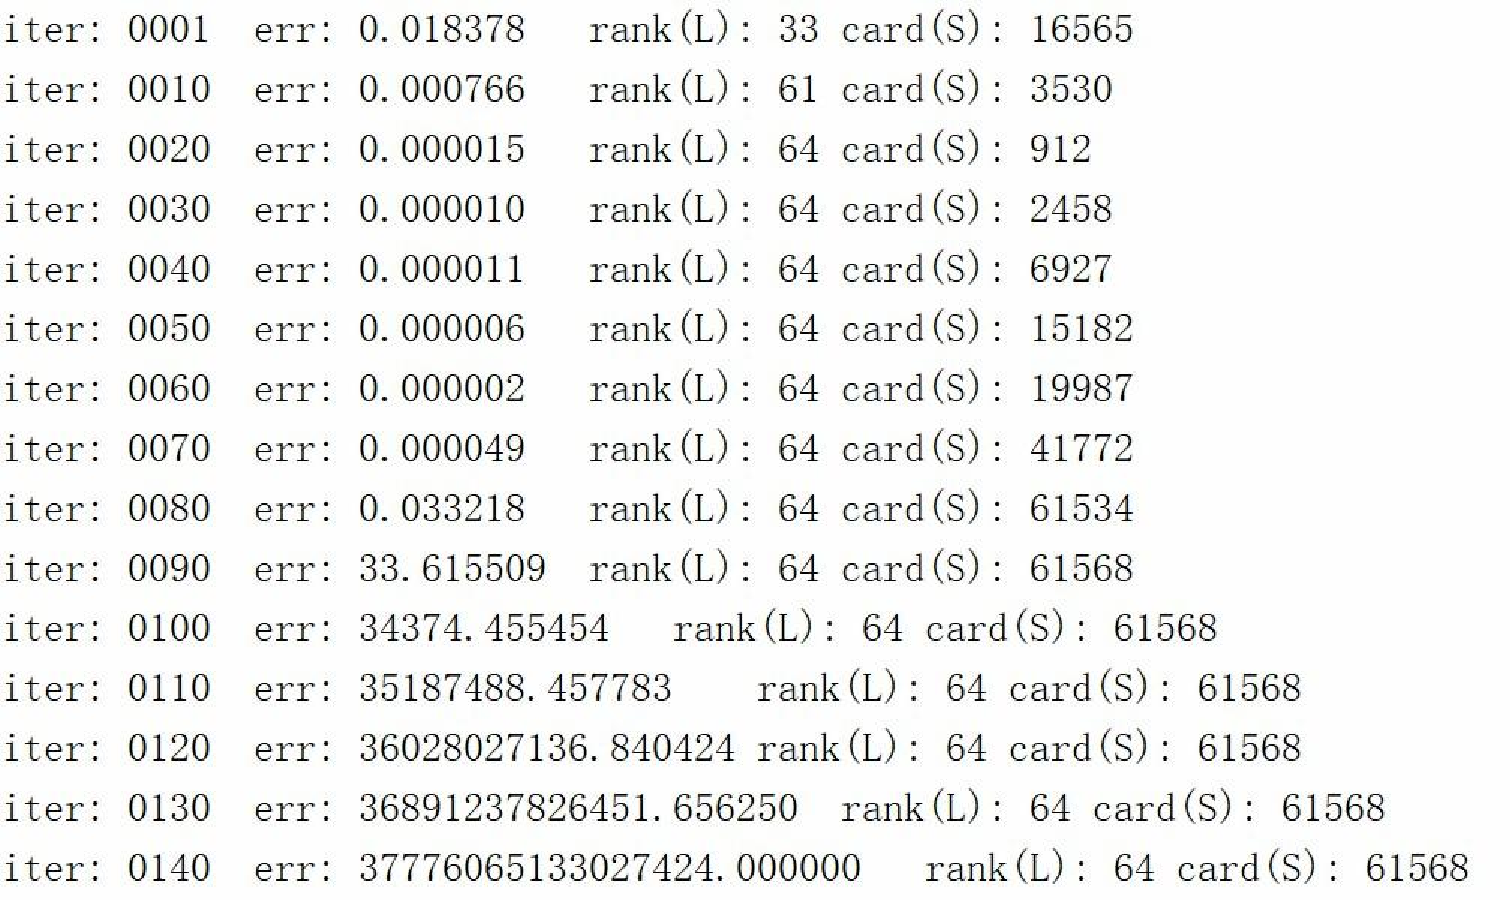
\includegraphics[width=0.70\textwidth]{explosion.pdf}
	\caption{Numerical result we got from the second image}
\end{figure}
And here we are showing the code we did in matlab:\\
\begin{lstlisting}
	clc
	clear
	
	addpath('../');
	
	img = double(imread('a.jpg'))/255;
	img2=double(imread('a_smd.png'))/255;
	img3 = double(imread('a.jpg'))/255;
	ws = 8; 
	a1=floor(size(img,1)/ws);
	b1=floor(size(img,2)/ws);
	img = img(1:a1*ws, 1:b1*ws);
	
	no_patches1 = size(img, 1) / ws;
	no_patches2 = size(img, 2) / ws;
	X = zeros(2,ws^2);
	k = 1;
	for i = (1:no_patches1)
	for j = (1:no_patches2)
	r1 = (i-1)*ws+1:i*ws;
	r2 = (j-1)*ws+1:j*ws;
	patch = img(r1, r2);
	X(k,:) = patch(:);
	k = k + 1;
	end
	end
	
	% apply Robust PCA
	lambda = 0.02; % close to the default one, but works better
	tic
	[L, S] = RobustPCA(X, lambda, 1.0, 1e-6);
	toc
	
	% reconstruct the image from the overlapping patches in matrix L
	img_low_rank = zeros(size(img));
	img_sparse = zeros(size(img));
	k = 1;
	for i = (1:no_patches1)
	for j = (1:no_patches2)
	patch = reshape(L(k,:), ws, ws);
	r1 = (i-1)*ws+1:i*ws;
	r2 = (j-1)*ws+1:j*ws;
	img_low_rank(r1, r2) = img_low_rank(r1, r2) + patch;
	patch = reshape(S(k,:), ws, ws);
	img_sparse(r1, r2) = img_sparse(r1, r2) + patch;
	k = k + 1;
	end
	end
	
	norm1=zeros(size(S,1),1);
	for i=1:size(S,1)
	for j=1:size(S,2)
	norm1(i,1)=norm1(i,1)+abs(S(i,j));
	end
	end
	
	S1=zeros(size(S));
	for i=1:size(S,1)
	if norm1(i)>=quantile(norm1,0.8,1)
	for j=1:size(S,2)
	S1(i,j)=255;
	end
	elseif (norm1(i)>=quantile(norm1,0.7,1))&&(norm1(i)<quantile(norm1,0.8,1))
	for j=1:size(S,2)
	S1(i,j)=175;
	end
	elseif(norm(i)>=quantile(norm1,0.6,1))&&(norm1(i)<quantile(norm1,0.7,1))
	for j=1:size(S,2)
	S1(i,j)=85;
	end
	else
	for j=1:size(S,2)
	S1(i,j)=0;
	end
	end
	end
	
	saliencemap=zeros(size(img));
	k=1;
	for i = (1:no_patches1)
	for j = (1:no_patches2)
	r1 = (i-1)*ws+1:i*ws;
	r2 = (j-1)*ws+1:j*ws;
	patch = reshape(S1(k,:), ws, ws);
	saliencemap(r1, r2) = saliencemap(r1, r2) + patch;
	k = k + 1;
	end
	end
	
	% show the results
	figure;
	subplot(2,3,1), imshow(img3,[]), title('Original')
	subplot(2,3,2), imshow(img_low_rank,[]), title('low rank image')
	bw_s = imbinarize(img_sparse,0.0000000001);
	bw_s=bw_s*255;
	subplot(2,3,3), imshow(bw_s), title('sparse image')
	subplot(2,3,4),imshow(saliencemap,[]),title('salience map')
	subplot(2,3,5),imshow(img2,[]),title('SMD result')
	fprintf(1, 'ws=%d\tlambda=%f\trank(L)=%d\tcard(S)=%d\terr=%f\n', ...
	ws, lambda, rank(L), nnz(S), norm(img - img_low_rank, 'fro'));
\end{lstlisting}
And here is the laplacian-matrix based LR-model function code:
\begin{lstlisting}
	function [L, S] = RobustPCA_laplacian(X, lambda, mu ,tol ,max_iter, beta)
	% - X is a data matrix (of the size N x M) to be decomposed
	%   X can also contain NaN's for unobserved values
	% - lambda - regularization parameter, default = 1/sqrt(max(N,M))
	% - mu - the augmented lagrangian parameter, default = 10*lambda
	% - tol - reconstruction error tolerance, default = 1e-6
	% - max_iter - maximum number of iterations, default = 1000
	
	[M, N] = size(X);
	unobserved = isnan(X);
	X(unobserved) = 0; 
	normX = norm(X, 'fro');
	
	% default arguments
	if nargin < 2 
	lambda = 1 / sqrt(max(M,N));
	end
	if nargin < 3
	mu = 10*lambda;
	end
	if nargin < 4
	tol = 1e-6;
	end
	if nargin < 5
	max_iter = 1000;
	end
	if nargin < 6
	beta=1.1;
	end
	
	% initial solution
	L = zeros(M, N);  %X=L+S
	S = zeros(M, N);
	Y1 = zeros(M, N);
	Y2 = zeros(M, N);
	w = zeros(M, M);
	MF =zeros(M, M);
	p=1.1;
	for i=1:M
	for j=1:M
	delta=norm(X(i,:)-X(j,:),'fro')/2;
	w(i,j)=exp(-delta);
	end
	end
	for i=1:M  
	for j=1:M
	if i~=j
	MF(i,j)=-w(i,j);
	end
	if i==j
	for k=1:M
	MF(i,j)=MF(i,j)+w(i,k);
	end
	MF(i,j)=MF(i,j)-w(i,j);
	end
	end
	end
	for iter = (1:max_iter)
	% ADMM step: update L and S
	L = Do(1/mu, X - S +1/mu*Y1); 
	H =(2*beta*MF+mu*eye(M))^(-1)*(mu*S+Y2);
	S = So(lambda/mu, X - L + (1/mu)*(Y1-Y2)+H); 
	% and augmented lagrangian multiplier
	Z = X - L - S;  
	Z(unobserved) = 0; % skip missing values
	Z1=S-H;
	Z1(unobserved) = 0;
	Y1 = Y1 + mu*Z; 
	Y2 = Y2 + mu*Z1;
	mu=p*mu;
	err = norm(Z, 'fro') / normX; 
	if (iter == 1) || (mod(iter, 10) == 0) || (err < tol)
	fprintf(1, 'iter: %04d\terr: %f\trank(L): %d\tcard(S): %d\n', ...
	iter, err, rank(L), nnz(S(~unobserved)));
	end
	if (err < tol)
	break; 
	end
	end
	end
	
	function r = So(tau, X)  
	% shrinkage operator
	r = sign(X) .* max(abs(X) - tau, 0);
	end
	
	function r = Do(tau, X)
	% shrinkage operator for singular values
	[U, S, V] = svd(X, 'econ');
	r = U*So(tau, S)*V'; 
	end
	
\end{lstlisting}
\section{Conclusion}
1.The result of LR model shows that the low rank matrix L is indeed low rank, but the sparse matrix s is not sparse enough.
\\2.After adding Laplacian to LR model, l is full rank and S is sparse (but sometimes it is too sparse).
\\3.LR model can effectively decompose the background and foreground, and the low rank matrix is especially good, but the sparse matrix is not sparse enough. After adding Laplacian, the low rank matrix is always full rank, and the effect is not good, but the sparse array retains the original spatial structure, which is particularly good for the foreground display of the image. However, sometimes it will be too sparse and cause the phenomenon of saliency image being prominent in the whole image.

\section{each one's work}
Yongqi Yuan\ :\ Mainly for computing and Latex part(50\%) \\
Ze Chen\ :\ Mainly for coding and Problem Statement part(50\%)
\bibliographystyle{plain}
\bibliography{references}
\end{document}
